\section{Projektvorgehen}

In dieser Arbeit wurde das Projektmanagement-Framework SCRUM eingesetzt, um ein möglichst
strukturiertes sowie flexibles Vorgehen zu gewährleisten. 
Die Entscheidung für SCRUM fielt dadurch dass es sich um eine
Softwareentwicklung handelt, bei der Anforderungen und Inhalte
häufig erst im Laufe des Projekts konkretisiert werden können.
SCRUM bietet hierfür einen geeigneten organisatorischen Rahmen,
um auf Änderungen reagieren zu können, ohne den gesamten
Projektplan neu ausarbeiten zu müssen \cite{dong2024}.

Wir haben auch GitHub genutzt, um Meilensteine und den Product Backlog zu managen. 
Als Versionsverwaltung hat es den Code gut im Griff gehalten und die Teamarbeit erleichtert. 
Mit Branches und Pull Requests konnten wir Änderungen tracken und checken, bevor sie reingingen. 
Das war praktisch, um nicht alles durcheinander zu bringen.

Agiles Projektmanagement eignet sich besonders für Projekte, wo erst
im Verlauf der Entwicklung Klarheit über Anforderungen und
Inhalte gewonnen wird.
Anstatt einer festen Planung von Anfang bis Ende, wie beim Wasserfallmodell, 
ermöglicht agiles Management eine flexible Anpassung an sich ändernde
Bedingungen \cite{kaack2016}.
In unserem Fall haben wir dadurch Zwischenergebnisse oft überprüft und angepasst, was die Plattform laufend besser gemacht hat. 
Das hat unseren Fortschritt beschleunigt und die Qualität des Ergebnis gesteigert.
\cite{dong2024}.

\subsection{SCRUM}

SCRUM ist ein Projektmanagement-Framework, das ursprünglich
für die Softwareentwicklung eingesetzt wurde.
Es basiert auf dem Schema von regelmäßigen Iterationen, den
Sprints, und fördert eine enge Zusammenarbeit im Team \cite{schwaber2020}.
Unter anderem gibt es festgelegte Rollen, die alle ihre spezifischen
Aufgaben und Verantwortlichkeiten haben.
Ziel von SCRUM ist es, das Projekt in überschaubare Abschnitte zu
unterteilen und durch regelmäßige Überprüfungen und Anpassungen
eine hohe Flexibilität zu gewährleisten \cite{schwaber2020}.

Der Sinn ist, das Ganze in kleine Teile zu brechen und flexibel zu bleiben durch Checks und Anpassungen.
Die Sprints dauern meist zwei bis vier Wochen, und am Start gibt es Planning, wo Ziele gesetzt werden. 
Am Ende dann Review, um zu sehen, was erreicht wurde.

SCRUM fördert die Selbstorganisation des Teams und legt großen Wert
auf Transparenz und kontinuierliche Verbesserung.
Es ist kein starrer Prozess, sondern ein flexibles Framework,
das an die spezifischen Bedürfnisse eines Projekts angepasst
werden kann.
Dadurch entsteht ein transparenter Prozess, bei dem alle
Beteiligten jederzeit Einblick in den aktuellen Entwicklungsstand
haben \cite{scrumguide2020}.

\subsection{Grundprinzipien von SCRUM}

SCRUM basiert auf mehreren grundlegenden Prinzipien, die im Projekt 
konsequent angewendet wurden.
Zu diesen Prinzipien wird Transparenz, Überprüfung und Anpassung gezählt. Diese
drei dominanten Prinzipien ermöglichen es eine herausragende Effizienzrate zu erzielen.

Doch was bedeuten diese Prinzipien im Detail?
Transparenz stellt sicher, dass alle Tätigkeiten, Prozesse und
Ergebnisse für alle Beteiligten klar und verständlich sind.
Überprüfung bedeutet, dass regelmäßig der Fortschritt und die
erreichten Ergebnisse genau betrachtet und überprüft werden.
Anpassung bedeutet, dass basierend auf Feedback und Überprüfungen
notwendige Änderungen am Projekt oder sämtlicher Prioritätenvorgenommen werden.
Durch diese 3er-Kombination wird eine hohe Flexibilität und
Effizienz im Projektmanagement gewährleistet \cite{schwaber2020}.

\subsection{Rollen im SCRUM}

SCRUM definiert drei zentrale Rollen, die gemeinsam für den Erfolg
des Projekts verantwortlich sind.
Diese Rollen sind der Product Owner, das Entwicklungsteam und der
Scrum Master \cite{scrumguide2020}.
Die klare Definition dieser Rollen trägt dazu bei, Verantwortlichkeiten
zu klären und eine effektive Zusammenarbeit im Team zu fördern.

\subsubsection{Product Owner}

Der Product Owner ist für die inhaltliche Ausrichtung des Projekts
verantwortlich.
Er priorisiert die Anforderungen im sogenannten Product Backlog
und stellt sicher, dass die umgesetzten Aufgaben den Bedürfnissen
der Nutzer:innen entsprechen \cite{schwaber2020}.
Im Projekt aber auch generell ist der Product Owner außerdem dafür
zuständig, Anforderungen zu präzisieren, Rückmeldungen aus dem Team
zu berücksichtigen und offene Fragen zu klären.
Anhand dieser Aufgaben sorgt der Product Owner dafür, dass das
Projekt zielgerichtet voranschreitet und die gewünschten Ergebnisse erarbeitet werden.

\subsubsection{Entwicklungsteam}

Das Entwicklungsteam setzte die geplanten Anforderungen um und
arbeitete selbstorganisiert.
Die Teammitglieder entscheiden eigenständig, welche Aufgaben
innerhalb eines Sprints umgesetzt werden können und wie diese
am besten realisiert werden \cite{schwaber2020}.
Diese Selbstorganisation fördert die Eigenverantwortung und die Motivation, da man sich aktiv in den Entwicklungsprozess einbringen kann.
\cite{kaack2016}.

\subsubsection{Scrum Master}

Der Scrum Master unterstützt das Team bei der Anwendung des
SCRUM-Frameworks.
Er achtet gezielt darauf, dass alle Termine eingehalten werden und organisiert die verschiedenen Meetings.
Außerdem sorgt er dafür, dass Hindernisse im Arbeitsprozess beseitigt werden.
Nicht zu verwechseln ist, dass der Scrum Master kein klassischer Projektleiter ist und somit keine direkten Anweisungen an das Team gibt.
\cite{scrumguide2020}.

\subsection{Ablauf eines SCRUM-Sprints}

Die Projektarbeit wird in mehrere zeitlich begrenzte Sprints
unterteilt.
Jeder Sprint beginnt mit einem Sprint Planning, in dem die Ziele
und Aufgaben für den kommenden Zeitraum festgelegt werden.
Die ausgewählten Aufgaben bilden das Sprint Backlog und
dienen als Grundlage für die Arbeit während des Sprints.

Während des Sprints arbeiteten die Teammitglieder an der Umsetzung
der definierten Aufgaben.
Regelmäßige Abstimmungen ermöglichten es, den aktuellen Stand
zu besprechen, Probleme frühzeitig zu erkennen und gemeinsam
Lösungen zu erarbeiten.

Am Ende jedes Sprints findet ein Sprint Review statt, bei dem die
umgesetzten Ergebnisse präsentiert und überprüft wurden.
Zusätzlich wird eine Sprint Retrospektive durchgeführt, um den
Arbeitsprozess zu reflektieren und Verbesserungsmöglichkeiten
für kommende Sprints zu identifizieren \cite{scrumguide2020}.

\begin{figure}[h]
    \centering
    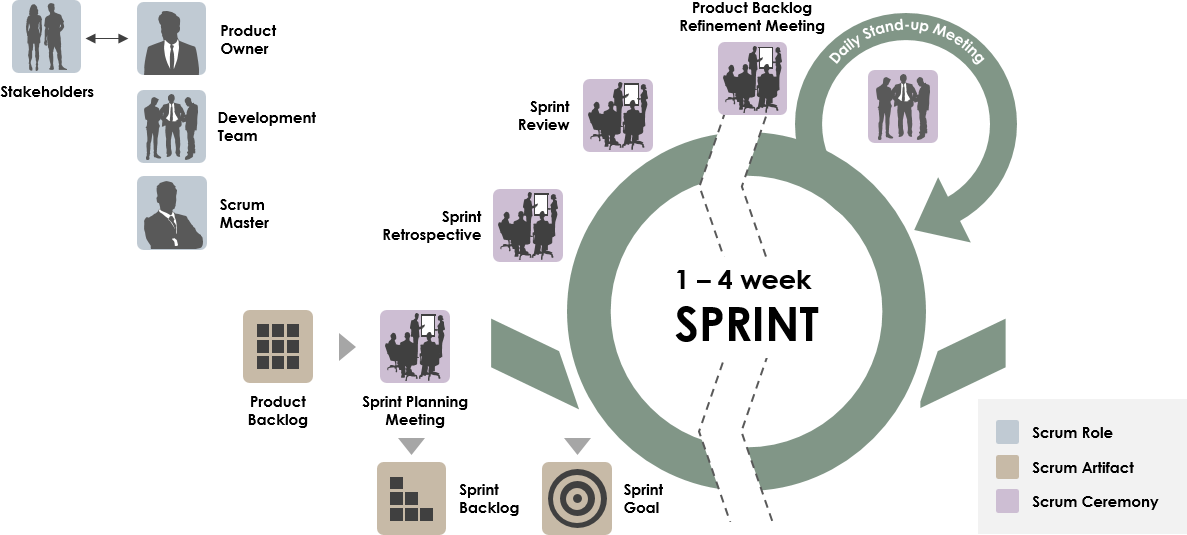
\includegraphics[width=0.95\textwidth]{pics/ScrumFramework.png}
    \caption{Ablauf eines SCRUM-Sprints}
    \label{fig:scrum_sprint}
\end{figure}

Abbildung~\ref{fig:scrum_sprint} zeigt den grundlegenden Ablauf
eines SCRUM-Sprints von der Planung über die Umsetzung bis hin
zum Review.

\subsection{Versionsverwaltung mit GitHub}

Zum generellen Management von Codeänderungen und zur Unterstützung
der Teamzusammenarbeit wird GitHub als Versionsverwaltungssystem
zur Verwaltung des Quellcodes und zur Unterstützung derTeamzusammenarbeit
eingesetzt.
GitHub ist eine webbasierte Plattform, die auf Git aufbaut.
Sie ermöglicht einen guten Überblick über die verschiedenen Versionen
des Codes sowie auch zahlreicher Dokumentationen \cite{tharu2025}.

Aufgrund der verteilten Natur von Git können mehrere Entwickler:innen
gleichzeitig am selben Projekt arbeiten, ohne sich gegenseitig zu behindern. 
Änderung, die lokal vorgenommen werden, können später in den zentralen Branch integriert werden.
Änderungen am Code werden in sogenannten Commits festgehalten,
die eine Beschreibung der vorgenommenen Änderungen enthalten. Somit ist es immer leicht nachvollziehbar, 
wer welche Änderungen vorgenommen hat \cite{sekery2020}.

Gezielt in unserem Projekt haben wir 3 Branches verwendet: den
Hauptbranch (main), einen Content-Management-Branch und einen Matura-Trainer-Branch.
Der Hauptbranch enthält den stabilen Code, während die
spezifischen Branches für die Entwicklung neuer Funktionen genutzt wurden.
Sobald ein Sprint abgeschlossen war, wurden die Änderungen auf den Mainbranch gemerged.
Dieser Workflow ermöglichte es, neue Funktionen zu entwickeln,
ohne die Stabilität des Hauptcodes zu gefährden \cite{tharu2025}

\begin{figure}[h]
    \centering
    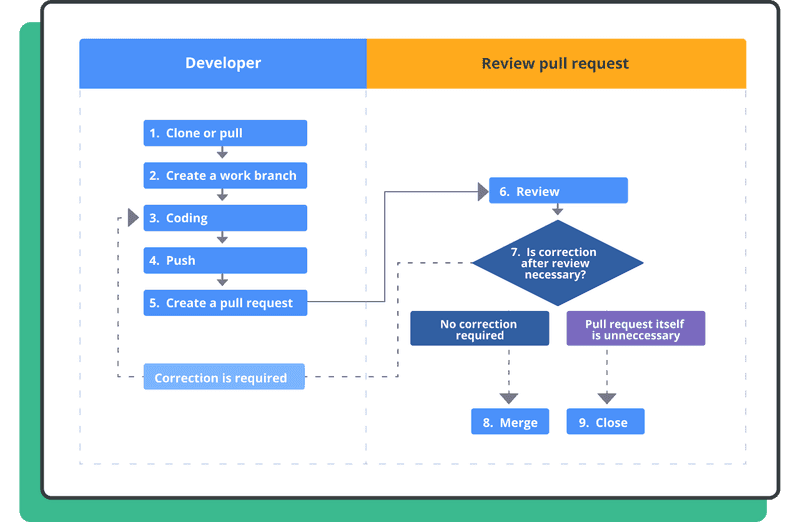
\includegraphics[width=0.95\textwidth]{pics/git-worflow.png}
    \caption{Vereinfachter GitHub-Workflow}
    \label{fig:github_workflow}
\end{figure}

Abbildung~\ref{fig:github_workflow} veranschaulicht den im Projekt
verwendeten GitHub-Workflow.

\subsection{Zusammenfassung}

Die Kombination von SCRUM als Projektmanagement-Framework und GitHub
als Versionsverwaltungssystem bildete die Grundlage für ein effizientes
und flexibles Projektvorgehen. Mit SCRUM konnten wir den Entwicklungsprozess
in überschaubare Sprints unterteilen, regelmäßige Überprüfungen und
Anpassungen vornehmen sowie eine enge Zusammenarbeit im Team fördern.
Github unterstützte uns dabei, den Quellcode effektiv zu verwalten,
Änderungen nachzuvollziehen und die Zusammenarbeit zu erleichtern.
Insgesamt trug dieses Vorgehen maßgeblich zum Erfolg des Projekts bei.